\section{Data} \label{sec:data}


In this paper I've selected 11 differenct stocks, to run my analysis on. The companies are:
\textit{Apple, General Electric, Boeing, Walmart, Coca Cola, JP Morgan Chase, Chevron, Cardinal Health, Exxon Mobile, IBM, Intel}. The companies have been chosen because they represent different sectors of the economy, and all of them have been going concerns for +30 years. The data covers the period: January 1990 to June 2019. The data consists of daily the Adjusted Close price. The data is acquired using a public API provided by \textit{Quandle}.

\begin{table}[ht]
\centering
\caption{Summary statistics of all 11 stocks}
\begin{tabular}{lrrrrrrrrrrr}
\toprule
{} &    AAPL &      GE &      BA &     WMT &      KO &     JPM &     CVX &     CAH &     XOM &     IBM &    INTC \\
\midrule
count &  7113.0 &  7114.0 &  7114.0 &  7114.0 &  7114.0 &  7114.0 &  7114.0 &  7114.0 &  7114.0 &  7114.0 &  7113.0 \\
mean  &    28.3 &    16.5 &    55.3 &    36.9 &    20.1 &    29.7 &    44.5 &    31.8 &    40.3 &    78.8 &    16.4 \\
std   &    43.0 &     8.7 &    53.0 &    22.5 &    11.4 &    21.5 &    34.5 &    22.0 &    27.4 &    52.6 &    10.8 \\
min   &     0.4 &     2.0 &    10.2 &     3.5 &     2.3 &     1.4 &     5.9 &     1.7 &     4.9 &     7.1 &     0.6 \\
25\%   &     1.2 &     8.8 &    23.5 &    10.7 &    14.1 &    14.6 &    16.4 &    14.3 &    14.8 &    26.1 &     9.9 \\
50\%   &     3.1 &    17.7 &    36.3 &    38.7 &    17.6 &    27.7 &    27.3 &    32.2 &    29.4 &    70.9 &    16.0 \\
75\%   &    43.2 &    23.4 &    64.2 &    46.0 &    26.7 &    36.3 &    72.7 &    39.4 &    67.0 &   123.9 &    21.5 \\
max   &   181.7 &    35.0 &   364.6 &   109.6 &    48.5 &   118.8 &   133.6 &    86.9 &    92.5 &   186.4 &    52.5 \\
\bottomrule
\end{tabular}

\label{tab:rawdata}
\end{table}

Table \ref{tab:rawdata} shows summary statistics of the raw data. On average 7114 observations is present for the total time period of 30 years. Figure \ref{fig:historicaltraces} presents all 11 traces. From this figure we can quickly deduce that the timeseries does not show stationarity, and in the long run follows an upward trend. For the analysis carried out in this paper, a transformation of the data is therefore necessary.
Instead of investigating stock prices, the focus will be on daily percentage change in stock prices. The summary statistics of this is shown in figure \ref{tab:cleandata}. Where the count of this now cleansed data is 7113. Additional to finding the percentage change of daily stock prices, rows containing NaN-values have been purged. In the appendix figure \ref{fig:returns_boxplots} shows the boxplot of the individual stocks expected daily return

\begin{figure}[ht]
\centering
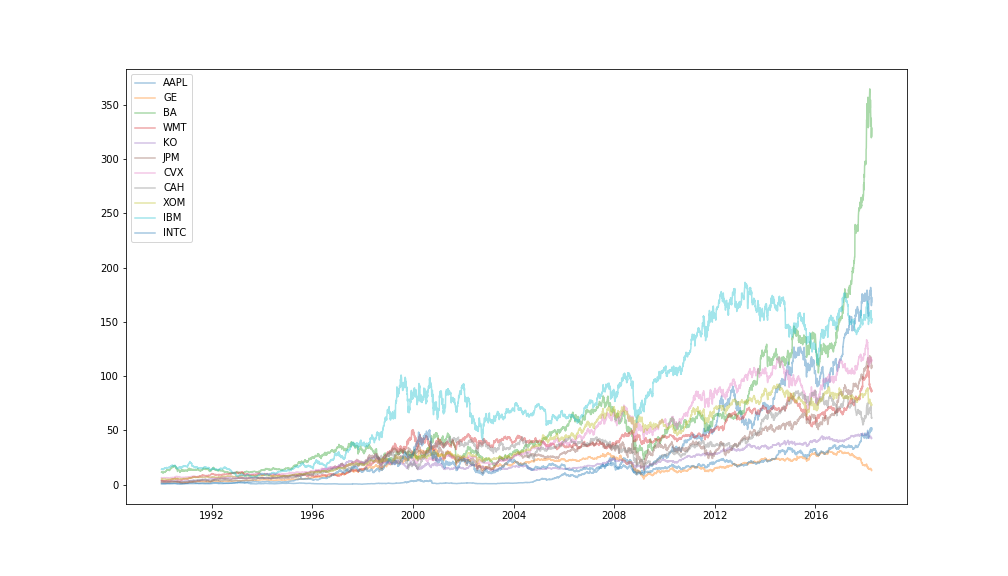
\includegraphics[scale=0.45]{figures/historicaltraces.png}
\caption{Historical trace plots of all 11 stocks}
\label{fig:historicaltraces}
\end{figure}

\begin{table}[ht]
\centering
\caption{Summary statistics of all 11 stocks, percentage change}
\begin{tabular}{lrrrrrrrrrrr}
\toprule
{} &    AAPL &      GE &      BA &     WMT &      KO &     JPM &     CVX &     CAH &     XOM &     IBM &    INTC \\
\midrule
mean &  0.0011 &  0.0004 &  0.0006 &  0.0006 &  0.0005 &  0.0008 &  0.0005 &  0.0007 &  0.0005 &  0.0005 &  0.0009 \\
std  &  0.0282 &  0.0175 &  0.0187 &  0.0165 &  0.0141 &  0.0241 &  0.0153 &  0.0188 &  0.0145 &  0.0174 &  0.0240 \\
min  & -0.5187 & -0.1279 & -0.1763 & -0.1018 & -0.1047 & -0.2073 & -0.1249 & -0.2454 & -0.1395 & -0.1554 & -0.2202 \\
25\%  & -0.0128 & -0.0079 & -0.0092 & -0.0079 & -0.0064 & -0.0101 & -0.0078 & -0.0084 & -0.0072 & -0.0079 & -0.0115 \\
50\%  &  0.0001 &  0.0000 &  0.0001 &  0.0000 &  0.0000 &  0.0000 &  0.0002 &  0.0000 &  0.0000 &  0.0001 &  0.0004 \\
75\%  &  0.0144 &  0.0087 &  0.0104 &  0.0087 &  0.0072 &  0.0107 &  0.0089 &  0.0097 &  0.0082 &  0.0087 &  0.0130 \\
max  &  0.3322 &  0.1970 &  0.1546 &  0.1107 &  0.1388 &  0.2510 &  0.2085 &  0.2039 &  0.1719 &  0.1316 &  0.2012 \\
\bottomrule
\end{tabular}

\label{tab:cleandata}
\end{table}

\subsection{Structural Breaks in the data}


This paper assumes that the underlying data generating process of the stock market experiences structural breaks. To confirm this whether or not the data display structural breaks we continue with a visual inspection of the expected returns and covariances of the returns.

Figure \ref{fig:structuralbreaksmeans} displays the bi-annual means of 4 stocks, these being Apple, General Electric, Boeing and Walmart. The displayed stocks are chosen randomly, and it is confirmed in the data that the same pattern is present in the other stocks. The figure shows the expected daily return on each of the stocks for a given year in the sequence: $1992, 1992, 1994, \cdots, 2018$. So for each of the calculated means, we have a one year period, where no mean is calculated. This is to avoid, that a possible structural break could be between two years an disturb the picture. This figure shows, as suspected, that the returns does not seem to adhere to the CAPM assumptions, of a single a vector of expected returns $\mu$, since this would imply that for each year each stock would have the approximately same expected return, which is not what the data displays. The same is true for the covariance matrix $\Omega$ which can be seen in the appendix figure \ref{fig:structuralbreakscovariances}.

\begin{figure}[ht]
\centering
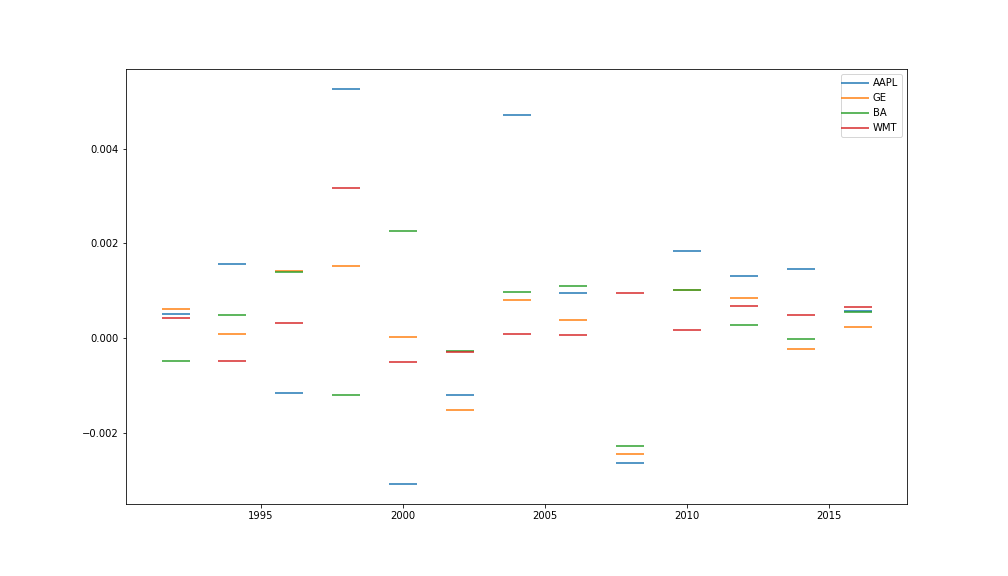
\includegraphics[scale=0.45]{figures/structural_breaks_means.png}
\caption{Bi-annual means of 4 stocks}
\label{fig:structuralbreaksmeans}
\end{figure}
